\documentclass[11pt]{amsart}


\usepackage[margin=1in]{geometry}
\usepackage{amsthm}
\usepackage{amsmath}
\usepackage{amssymb}
\usepackage{enumerate}
\usepackage[inline]{enumitem}
\usepackage{bbm}

\usepackage{tikz}
\usetikzlibrary{calc}
\usetikzlibrary{shapes}
\usetikzlibrary{positioning}

\newcommand\cH{{\mathcal H}}
\newcommand{\Prob}[1]{\ensuremath{%
    \mathbb P\left[#1\right]
}}
\newcommand{\ProbCond}[2]{\ensuremath{%
    \mathbb P\left[#1\:\middle|\:#2\right]
  }}
\newcommand{\Expect}[1]{\ensuremath{%
    \mathbb E\left[#1\right]
  }}

\newtheorem*{theorem*}{Theorem}
\newtheorem*{lemma*}{Lemma}
\theoremstyle{definition}
\newtheorem{problem}{Problem}[]
\newtheorem{exercise}{Exercise}[]
\newtheorem*{definition*}{Definition}


\title[Math 4032: Homework \#4\qquad Due March 10 at 1:59pm]{Math 4032: Homework \#4\\
  Due March 10 at 1:59pm}


\begin{document}


\maketitle

The relevant background material for this assignment is covered in Chapters 3 and 4 of the Jukna book and Chapters 10 and 11 of the Matou\v{s}ek--Ne\v{s}et\v{r}il book.  Techniques to be used in this assignment include the Pigeonhole Principle and the Probabilistic Method.
%\noindent\textit{Instructions:}
\begin{itemize}
\item You are strongly encouraged to typeset your homework solutions using \LaTeX.
\item Acknowledge collaborations as noted in the syllabus.
\item The following problems are optional exercises not to be turned in.  Problems to be turned in for a grade begin on the next page.  
\end{itemize}


\begin{exercise}
  Prove that $R(3, 3) = 6$ and $R(3, 4) \leq 9$.  \textit{Try to find a short proof!}  Prove that $R(4, 4) = 18$.  \textit{Hint: Use the fact from class that $R(s, t) \leq R(s - 1, t) + R(s, t - 1)$ to prove that $R(4, 4) \leq 18$, and prove $R(4, 4) \geq 18$ using the graph below.}
\end{exercise}

\begin{center}
  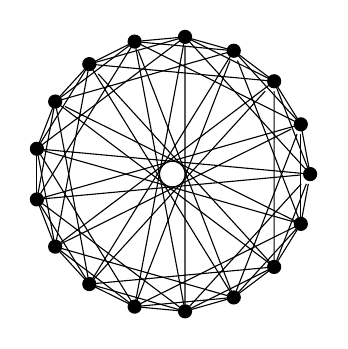
\begin{tikzpicture}
    \tikzstyle{vtx}=[draw, fill, circle, scale=.5];
    \pgfmathsetmacro{\rad}{1.75}
    \foreach \i in {0,...,16} {
      \node[vtx] (\i) at (\i*360/17:\rad) {};
    }
    \foreach \i in {17,...,33} {
      \node (\i) at (\i*360/17:\rad) {};
    }
    \foreach \i in {0,...,16} {
      \foreach \j in {1, 2, 4, 8} {
        \pgfmathtruncatemacro{\k}{\i+\j}
        \draw (\i) -- (\k);
      }
    }
  \end{tikzpicture}
\end{center}

\begin{exercise}
  Prove that for all $r, k, s_1, \dots, s_{r+1} \in \mathbb N$,
  \begin{equation*}
    R_r(s_1, \dots, s_{r+1}; k) \leq R_r(s_1, \dots, s_{r-1}, R_2(s_r, s_{r+1}; k); k),
  \end{equation*}
  and complete the proof of the Hypergraph Ramsey Theorem.  
\end{exercise}

\begin{exercise}
  Prove that if $A$ and $B$ are independent events in a probability space $(\Omega, \mathbb P)$, then $\Omega\setminus A$ and $\Omega \setminus B$ are also independent.
\end{exercise}

\begin{exercise}
  Construct a probability space and three events which are pairwise independent but not mutually independent.  (That is, find events $A_1$, $A_2$, and $A_3$ such that $A_i$ and $A_j$ are independent for all $\{i, j\} \in \binom{[3]}{2}$ but $A_1$, $A_2$, and $A_3$ are not mutually independent.)
\end{exercise}

\begin{exercise}
  Construct examples of random variables $X$ and $Y$ such that
  \begin{itemize}
  \item $\Expect{XY} \neq \Expect{X}\Expect{Y}$,
  \item $\Expect{X^2} \neq \Expect{X}^2$,
  \item $\Expect{1/X} \neq 1 / \Expect{X}$,
  \end{itemize}
  and prove that $\Expect{XY} \geq \Expect{X}\Expect{Y}$ for every pair of random variables $X$, $Y$.
\end{exercise}
\clearpage

\begin{problem}
  Let $n \in \mathbb N$ and $r \in [n - 1]$.  Prove that if $\chi : [n] \rightarrow [r]$ is an $r$-coloring of $[n]$, then
  \begin{equation*}
    \left|\left\{\{i, j\} \in \binom{[n]}{2} : \chi(i) = \chi(j)\right\}\right| \geq  \frac{n(n - 1)}{(r + 1)r}. 
  \end{equation*}
\end{problem}

\begin{proof}
Let assumptions be as in the problem statement, that is to say that we have an $r$-coloring on $n$ elements and we are looking to find the lower bound on the number of pairs in this coloring mapping $\{i, j\}$ such that $\chi(i) = \chi(j)$, i.e. the elements of the pairs map to the same coloring. Let us consider a subset of size $r + 1$ from the set $[n]$, since this is an $r$-coloring, since we have $r + 1$ elements, by the pigeonhole principle that means we must have one such pair in this subset. If we consider this for all subsets of size $r + 1$, of which there are $\binom{n}{r+1}$ of, we will get some double counting. Then we know that the number of times each of these pairs will be double counted is given by $\binom{n-L}{r+1 - L}$ where for this scenario, since we are counting pairs, $L = 2$, which makes this then $\binom{n-2}{r-1}$. If we then divide this out from the total number of subsets, we get $\frac{\binom{n}{r+1}}{\binom{n-2}{r-1}} = \frac{\frac{n!}{(r+1)!(n-r-1)!}}{\frac{(n-2)!}{(r-1)!(n-r-1)!}} = \frac{n!(r - 1)!(n - r - 1)!}{(r+1)!(n - r - 1)!(n - 2)!} = \frac{n(n-1)}{r(r+1)}$. Thus we find that the number of these pairs is $\geq \frac{n(n - 1)}{(r + 1)r}$ as desired.
\end{proof}

\clearpage
\begin{problem}~
  \begin{enumerate}[label={(\alph*)}]
  \item Let $s, t, n \in \mathbb N$.  Prove that, if there exists $p \in [0, 1]$ such that
    \begin{equation*}
      \binom{n}{s}p^{\binom{s}{2}} + \binom{n}{t}(1 - p)^{\binom{t}{2}} < 1,
      \end{equation*}
      then $R(s, t) > n$.

\begin{proof}
    Let assumptions be as in the problem statement. Let us randomly color each of the $n$ edges red with probability $p$ or blue otherwise ($1-p$). Then it follows that the probability of having a red $K_s$ or a blue $K_t$ is at most $\binom{n}{s}p^{\binom{s}{t}} + \binom{n}{t}(1-p)^{\binom{t}{2}} < 1$. Since this is a strict inequality (no equality), then we know that in order to guarantee to have a $K_s$ or a $K_t$ then we know we must have more than $n$ points. Thus given this, we know that $R(s, t) > n$ as desired.
\end{proof}
      
    \item Prove that
      \begin{equation*}
        R(4, t) = \Omega\left(\frac{t^{3/2}}{(\ln t)^{3/2}}\right).
      \end{equation*}

\begin{proof}
    Let assumptions be as above. We will note that $\binom{n}{s}p^{\binom{s}{2}} + \binom{n}{t}(1-p)^{\binom{t}{2}} < n^sp^{\binom{s}{2}}/s! + n^te^{-\binom{t}{2}p}/b!$. Then if we allow that $n^sp^{\binom{s}{2}}/s!\leq 1/2$ and $n^te^{-\binom{t}{2}p}/t! \leq 1/2$ then we will maintain the findings from part a. This is the same thing as saying that $p \leq \frac{(s!/2)^{1/\binom{s}{2}}}{n^{2/(s - 1)}}$ and $p \geq \frac{\ln(t!/(2n^t))}{\binom{t}{2}}$, which then implies that $\frac{\ln(t!/(2n^t))}{\binom{t}{2}} \leq \frac{(s!/2)^{1/\binom{s}{2}}}{n^{2/(s - 1)}}$ for large enough $n.$ So if we plug in $s = 4$ and simplify we get that $n = \Omega\left(\frac{t^{3/2}}{(\ln{t}^{3/2}}\right)$ as desired.
\end{proof}
      
  \end{enumerate}
\end{problem}

\clearpage
\begin{problem}
  Let $(\Omega, \mathbb P)$ be a finite probability space, and let $A_1, \dots, A_n$ be events in $\Omega$.  Prove that
  \begin{equation*}
    \Prob{\bigcup_{i=1}^nA_i} \leq \sum_{k=1}^\ell (-1)^{k-1}\sum_{I \in \binom{[n]}{k}}\Prob{\bigcap_{i \in I}A_i} \text{ for every odd } \ell \in [n]
  \end{equation*}
  and
  \begin{equation*}
    \Prob{\bigcup_{i=1}^nA_i} \geq \sum_{k=1}^\ell (-1)^{k-1}\sum_{I \in \binom{[n]}{k}}\Prob{\bigcap_{i \in I}A_i} \text{ for every even } \ell \in [n].
  \end{equation*}
  The case $\ell = 1$ is referred to as the \textit{Union Bound}.
\end{problem}

\begin{proof}
    Let assumptions be as in the problem statement, and let us define an indicator function $\mathbbm{1}$ for which it is only equal to $1$ when an $\omega$ belongs to each of $A_{i_1}\cap ... \cap A_{i_j}$ and we will define $T = \sum_{i = 1}^n \mathbbm{1}(A_i)$ which means that the expected value of $\sum_{i_1 < ... < i_j} \mathbbm{1}(A_{i_1}\cap ... \cap A_{i_j}) = \binom{T}{j}$ because the LHS of this equation counts the number of ways to select $j$ $A$s for which $\omega$ belongs and the RHS is the same thing as a binomial and we will define this expected value to be $S_j$. This then allows us to redefine the problem to be $\Prob{\bigcup_{i = 1}^nA_i} + \sum_{j = 1}^k(-1)^jS_j \leq 0$ when $k$ is odd and $\geq 0$ when $k$ is even. Then we find the expected value of $\mathbbm{1}(\bigcup A_i) + \sum_{j = 1}^k(-1)^j\binom{T}{j} = \mathbbm{1}(\bigcup A_i) \left[ \sum_{j = 0}^k(-1)^j \binom{T}{j}\right] = \mathbbm{1}(\bigcup A_i)\left[(-1)^k\binom{T-1}{k}\right]$ which implies that this is negative when $k$ is odd and positive when $k$ is even which is as desired for the problem statement.
\end{proof}

NOTE: This is the proof I had the hardest time on, do you think you can release the solution to this one? My friend told me the TA said this one could be done through induction, but I had a hard time seeing that solution. I understood to do induction on $\ell$ and to separate the sum into $\sum_{k = 1}^{\ell - 1} + (-1)^{\ell - 1}$ term and to apply inductive hypothesis on the $\ell - 1$ term in the first sum, which would then mean that we need to prove that the $\ell$ term would need to flip the sign of the probability. This is where I was having the difficulty in flipping the sign to show that it changes the parity of the probability of the big union. Maybe this is where I could use the indicator function on that last term to show that it would have a positive value so if it is subtracted it would flip the sign or maybe if it is added it would flip the sign the other way? Thanks! 

\clearpage
\begin{problem}
  Let $k, n \in \mathbb N$, and let $\ell = \lceil 2k 4^k \ln n\rceil$.  Prove that there exist $Y_1, \dots, Y_\ell \subseteq [n]$ such that every pair of disjoint $A, B \in \binom{[n]}{k}$ satisfies
  \begin{equation}\tag{$\dagger$}\label{eq:separation}
    A \subseteq Y_i \text{ and } B \cap Y_i = \varnothing \text{ for some } i \in [\ell].
  \end{equation}
  \textit{Hint: Choose $Y_1, \dots, Y_\ell$ randomly and independently and show that \eqref{eq:separation} holds with probability at least $1 - (1 - 2^{-2k})^\ell$.  Use that $1 + x \leq e^x$ and the Union Bound from the previous problem.}
\end{problem}

\begin{proof}
    Let assumptions be as in the problem statement. Let us choose $Y_1, ..., Y_\ell \subseteq [n]$ at random and independently from each other. Then in order for \eqref{eq:separation} we need for particular $Y_i$ to contain all $k$ elements of $A$ and not to contain all elements of $B$ which means the probability for this is $\frac{1}{2^k} * \frac{1}{2^k} = \frac{1}{2^{2k}}$. So let us consider when this $Y_i$ would not meet the requirements for a particular $A, B$ would be $(1-2^{-2k})$ and for this to be true for all $\ell$ $Y_i$s we would have $(1-2^{-2k})^\ell$. However, this is for a particular pair $A, B$ so we instead need to consider for all $A, B$ for which there are $\binom{n}{k}\binom{n - k}{k} < n^{2k}$ such $A, B.$ So, by the union bound, the probability that this fails for at least one $A, B$ is $\leq \binom{n}{k}\binom{n-k}{k}(1-2^{-2k})^\ell < n^{2k}(1-2^{-2k})^\ell < n^{2k}(e^{-2^{-2k}})^\ell = n^{2k}e^{\frac{-\ell}{2^2k}}$. We will want to show that this probability is less than one, i.e. we need to show that $e^{\frac{-\ell}{2^{2k}}} < \frac{1}{n^{2k}}$. So it follows that we need $\frac{-\ell}{2^{2k}} < -\ln{{n^{2k}}} \Rightarrow \frac{\ell}{2^{2k}} > 2k\ln{n} \Rightarrow \ell > 2k4^k\ln{n}$ and then it would suffice that $\ell = \lceil 2k4^k\ln{n}\rceil$ which it is as defined in the problem. Thus, since this probability is not equal to 1, we know then that there does in fact exist some $Y_i$ such that for every disjoint $A, B$ it satisfies \eqref{eq:separation} as desired. 
\end{proof}

\clearpage
A hypergraph is \textit{$k$-uniform} if its edges all have size $k$; that is, $\cH = (V, E)$ is $k$-uniform if $E \subseteq \binom{V}{k}$.  Note that graphs are $2$-uniform.
\begin{problem}
  Let $k,r \in \mathbb N_{\geq 2}$, and let $\cH = (V, E)$ be a $k$-uniform hypergraph.  Prove that if $|E| \leq r^{k - 1}$, then there is an $r$-coloring $\chi : V \rightarrow [r]$ such that no edge of $\cH$ is monochromatic (that is, there exist $u, v \in e$ such that $\chi(u) \neq \chi(v)$ for every $e \in E$).  \textit{Hint: Consider a random coloring and compute the expected number of monochromatic edges.}
\end{problem}

\begin{proof}
    Let assumptions be as in the problem statement. Let us randomly color the vertices of the graph $\cH$ with any color $[r]$ and since $\cH$ is $k$-uniform we know that each edge is incident on $k$ vertices. Let us define an indicator function $\mathbbm{1}_m$ which we will define as equal to $1$ when the edge is monochromatic. Therefore if we find the expected value of this indicator function as follows $\mathbb{E}[\sum_{e\in E}\mathbbm{1}(e)$ which we can then modify by the linearity of expectation to get $\sum_{e\in E}\mathbb{E}[\mathbbm{1}] = \sum_{1}^{|E|}\mathbb{P}(\text{edge i is monochromatic}) = \sum_{e\in E}\frac{r}{r^k}$ as each vertex has $\frac{1}{r}$ probability to be colored each color, which is then equal to $\frac{|E|}{r^{k-1}}$. We then want the expectation to be less than $1$ so that by the pigeonhole principle for expectations there would exist a coloring with $<1 \Rightarrow0$ monochromatic edges. Then we have that $|E| < r^{k - 1}$, but if the expected value of the number of monochromatic edges is $\leq r^{k-1}$ and there exists a coloring with $> r^{k - 1}$ monochromatic edges, then there exists a coloring with $< r^{k - 1}$ monochromatic edges. Thus we can say that if $|E| \leq r^{k - 1}$ then there exists an $r$-coloring such that no edge in $\cH$ is monochromatic as desired. 
\end{proof}

\end{document}

%%% Local Variables:
%%% mode: latex
%%% TeX-master: t
%%% End:
